\chapter{Implementation-1}
\label{ch:implementation}
\section*{Part 1}
\label{sec:implemenation:part1}
\section{Camera Calibration}
\label{sec:camcalib}
Cameras in real life introduce significant amount of distortion to the images due to internal or external influences. There are 2 types of distortions – Tangential distortion and Radial distortion. Radial distortion makes the straight lines in the image to be curved. Tangential distortion takes place when the lens of the camera is not aligned parallel to the sensor plane. Due to this the image appears to be closer than in reality. To overcome these errors, camera calibration is done to obtain the distortion coefficients, camera matrix and other necessary camera data rectify the distorted image.\\

ORBSLAM3 takes in a yaml settings file that specifies camera intrinsic parameters, distortion parameters and ORB parameters. We can extract intrinsic and distortion parameters from camera calibration process.
ROS contains out-of-box camera calibrator python script which allows the user to calibrate the camera.  The below command is use to carry out the calibration process in ROS.
\begin{lstlisting}[language=bash, basicstyle=\small]
$ roscore
$ rosrun camera_calibration cameracalibrator.py  
- -size 8x6 - -square 0.075 image:=/dji_osdk_ros/main_camera_images  camera:=/camera
\end{lstlisting} 

So obtained parameters from this calibration was updated into the settings file for the ORBSLAM3.

\section{vid\_orbslam3 package for Visual SLAM}
\label{sec:initialpackagevslam}
The package vid\_orbslam3 was developed as a ROS package to create a node that subscribes to a camera image topic and perform monocular visual SLAM for each image frame. ORBSLAM3 library provides definite methods which can be used to initiate and perform monocular SLAM through our node. The ORBSLAM system object is instantiated as a monocular functioning entity. Since ORBSLAM3 uses pangolin for the visualization, it is impractical to use visualization on a headless Manifold 2. However, the display of the visualization can be switched on/off with our node for specific usage if a monitor is connected for debugging. Some utilities that were developed as part of this task are as follows -
\begin{itemize}
    \item Method that stores the camera intrinsic and distortion parameters for usage.
    \item Method that performs Hamilton product between 2 quaternions.
\end{itemize}
The node takes in vocabulary file and settings file as input that contributes information for keypoint detection and pose estimation. ORBSLAM3 system class provides method named as \emph{System::TrackMonocular} for performing monocular SLAM tracking. For every image frame, the above method returns a camera pose matrix \((^wT_c)\) in orbslam coordinate system. The entity or object created before is used for the invocation of the above tracking method. The camera poses returned are transformed into ROS coordinate system with rotation matrix \((^{ros}R_{orb})\) and published as a pose topic. Alternatively, the pose can also be broadcast as a transform or TF.

\begin{align}
   ^{ros}R_{orb} =
   \begin{bmatrix}
   0 & 0 & 1\\
  -1 & 0 & 0\\
   0 & -1 & 0
   \end{bmatrix}
\end{align}

The node was tested using a pre-recorded rosbag recorded using the drone and we were able to visualize the pose on Rviz. Nevertheless, the results are not acceptable until tested in real-time. For this the drone has to be made as a slave and a local PC as master for the real-time camera pose visualization. In the next section, a brief explanation is given about the ROS master-slave setup.

\section{ROS master-slave setup}
\label{sec:masterslavesetup}
In real-time, visualization of camera pose plays important role for UAV based SLAM implementations. ROS solves the problem of remote visualization with it's master-slave functionality. This setup requires both the drone and the local PC to be connected to same local network. Run the following linux commands in the working terminal for both master (loacl PC) and slave (Manifold 2)-\\
\\
Master side:
\begin{lstlisting}[language=bash, basicstyle=\small]
$ export ROS_MASTER_URI=http://<IP-addr-of-master>:11311/
$ export ROS_HOSTNAME=<IP-addr-of-master>
\end{lstlisting}
Slave side:
\begin{lstlisting}[language=bash, basicstyle=\small]
$ export ROS_MASTER_URI=http://<IP-addr-of-master>:11311/
$ export ROS_HOSTNAME=<IP-addr-of-slave>
\end{lstlisting}

If multiple terminals are used for execution, for uniformity, add these lines into respective .bashrc files. After this, both the systems are ready for master-slave functionality.

\section{Drone flight and vid\_orbslam3 node}
\label{sec:droneflight}
The drone and the local system was setup as explained before and  vid\_orbslam3 node was launched using a ros launch file. As expected, we obtained real-time camera poses through the published rostopics. The visualization was made using Rviz tool on the local PC. But it was observed that monocular SLAM resets the map and tracking when the vehicle moves too quickly. This affects the motion of the camera and hence will not allow monocular SLAM system to detect keypoints in turn punishes the pose estimation process. A similar observation in an article \cite{Luo2020} was reported for poor feature point extraction and system tracking failure due to motion blur caused by quick camera rotation or movements at large angles.

\subsection*{Need for Visual Inertial SLAM}
Interestingly, it was also found that Visual SLAM has scale ambiguity and is suitable for indoor environments. To overcome this, stereo cameras are used for the correction. For catering single camera setup, IMU fusion with the camera resolves the scale ambiguity. This results in Visual Inertial SLAM. ORBSLAM3 offers VI-SLAM as a new add-on from it's previous release ORBSLAM2. Hence, VI-SLAM is suitable for both indoor and outdoor environments. IMU measurements can provide quick velocity and absolute scale information ramping up the estimation process as explained in \cite{7487266}.

\section{IMU calibration and T\textsubscript{bc} estimation}
\label{sec:imucalib}
ORBSLAM3 library offers Visual Inertial SLAM as mentioned in the previous section \ref{sec:droneflight}. The SLAM settings file for VI-SLAM extends Visual SLAM settings file and requires IMU intrinsic parameters and extrinsic parameters or transformation matrix from body to camera \((T_{bc})\) as additional information. Camera pose estimation in case of VI-SLAM takes IMU measurements into consideration. A pose estimation may fail or can have induced error if the intrinsic parameters are not accurate. This process is very much sensitive on IMU intrinsic parameters which boils down to the order of 10\textsuperscript{-4} or sometimes even lower depending on the quality of the IMU sensor.\\

IMU intrinsic parameters consists of 2 values: Additive White Noise (AWN) and Bias also termed as random walk. These two parameters are applicable for both accelerometer and Gyroscope of the IMU module. Therefore, a set of IMU intrinsic parameters has 4 values to be measured. The below equation is the IMU noise model presented by the Kalibr \cite{Kalibr}.

\begin{equation}
    \Tilde{\omega}(t) = \omega(t) + b(t) + n(t) 
\end{equation}

where $\Tilde{\omega}$(t) denotes angular rate measurement, $\omega$(t) denotes actual angular rate, b(t) is random walk or bias and n(t) is additive white noise of one single axis of gyroscope. This equation applies to other axes as well as for the accelerometer. \\

Our drone is considered as an autonomous aerial robot whose motion and attitude are agile. Some of the VI-SLAM implementations provide online IMU intrinsic parameter calculation. But findings presented by Yang et al. \cite{Yang2020} explains the observability of all the 6 axes of IMU sensor while calculating the intrinsic parameters online and why offline calibration is still effective in the case of autonomous robot like environment.

\subsection*{Calibrating IMU intrinsic parameters}
To calculate the intrinsic parameters, additive white noise and random walk, a 2-hour rosbag was recorded containing IMU ros topic /dji\_osdk\_ros/imu from the drone. In the DJI Matrice 210 RTK v2, the IMU sensor is set to publish fused data at 400 Hz. Good results are achieved when calibrated using raw data. Therefore, we used the drone's pilot to change the IMU sensor publish mode to raw data at 400 Hz. 

\begin{figure}[h]
    \centering
    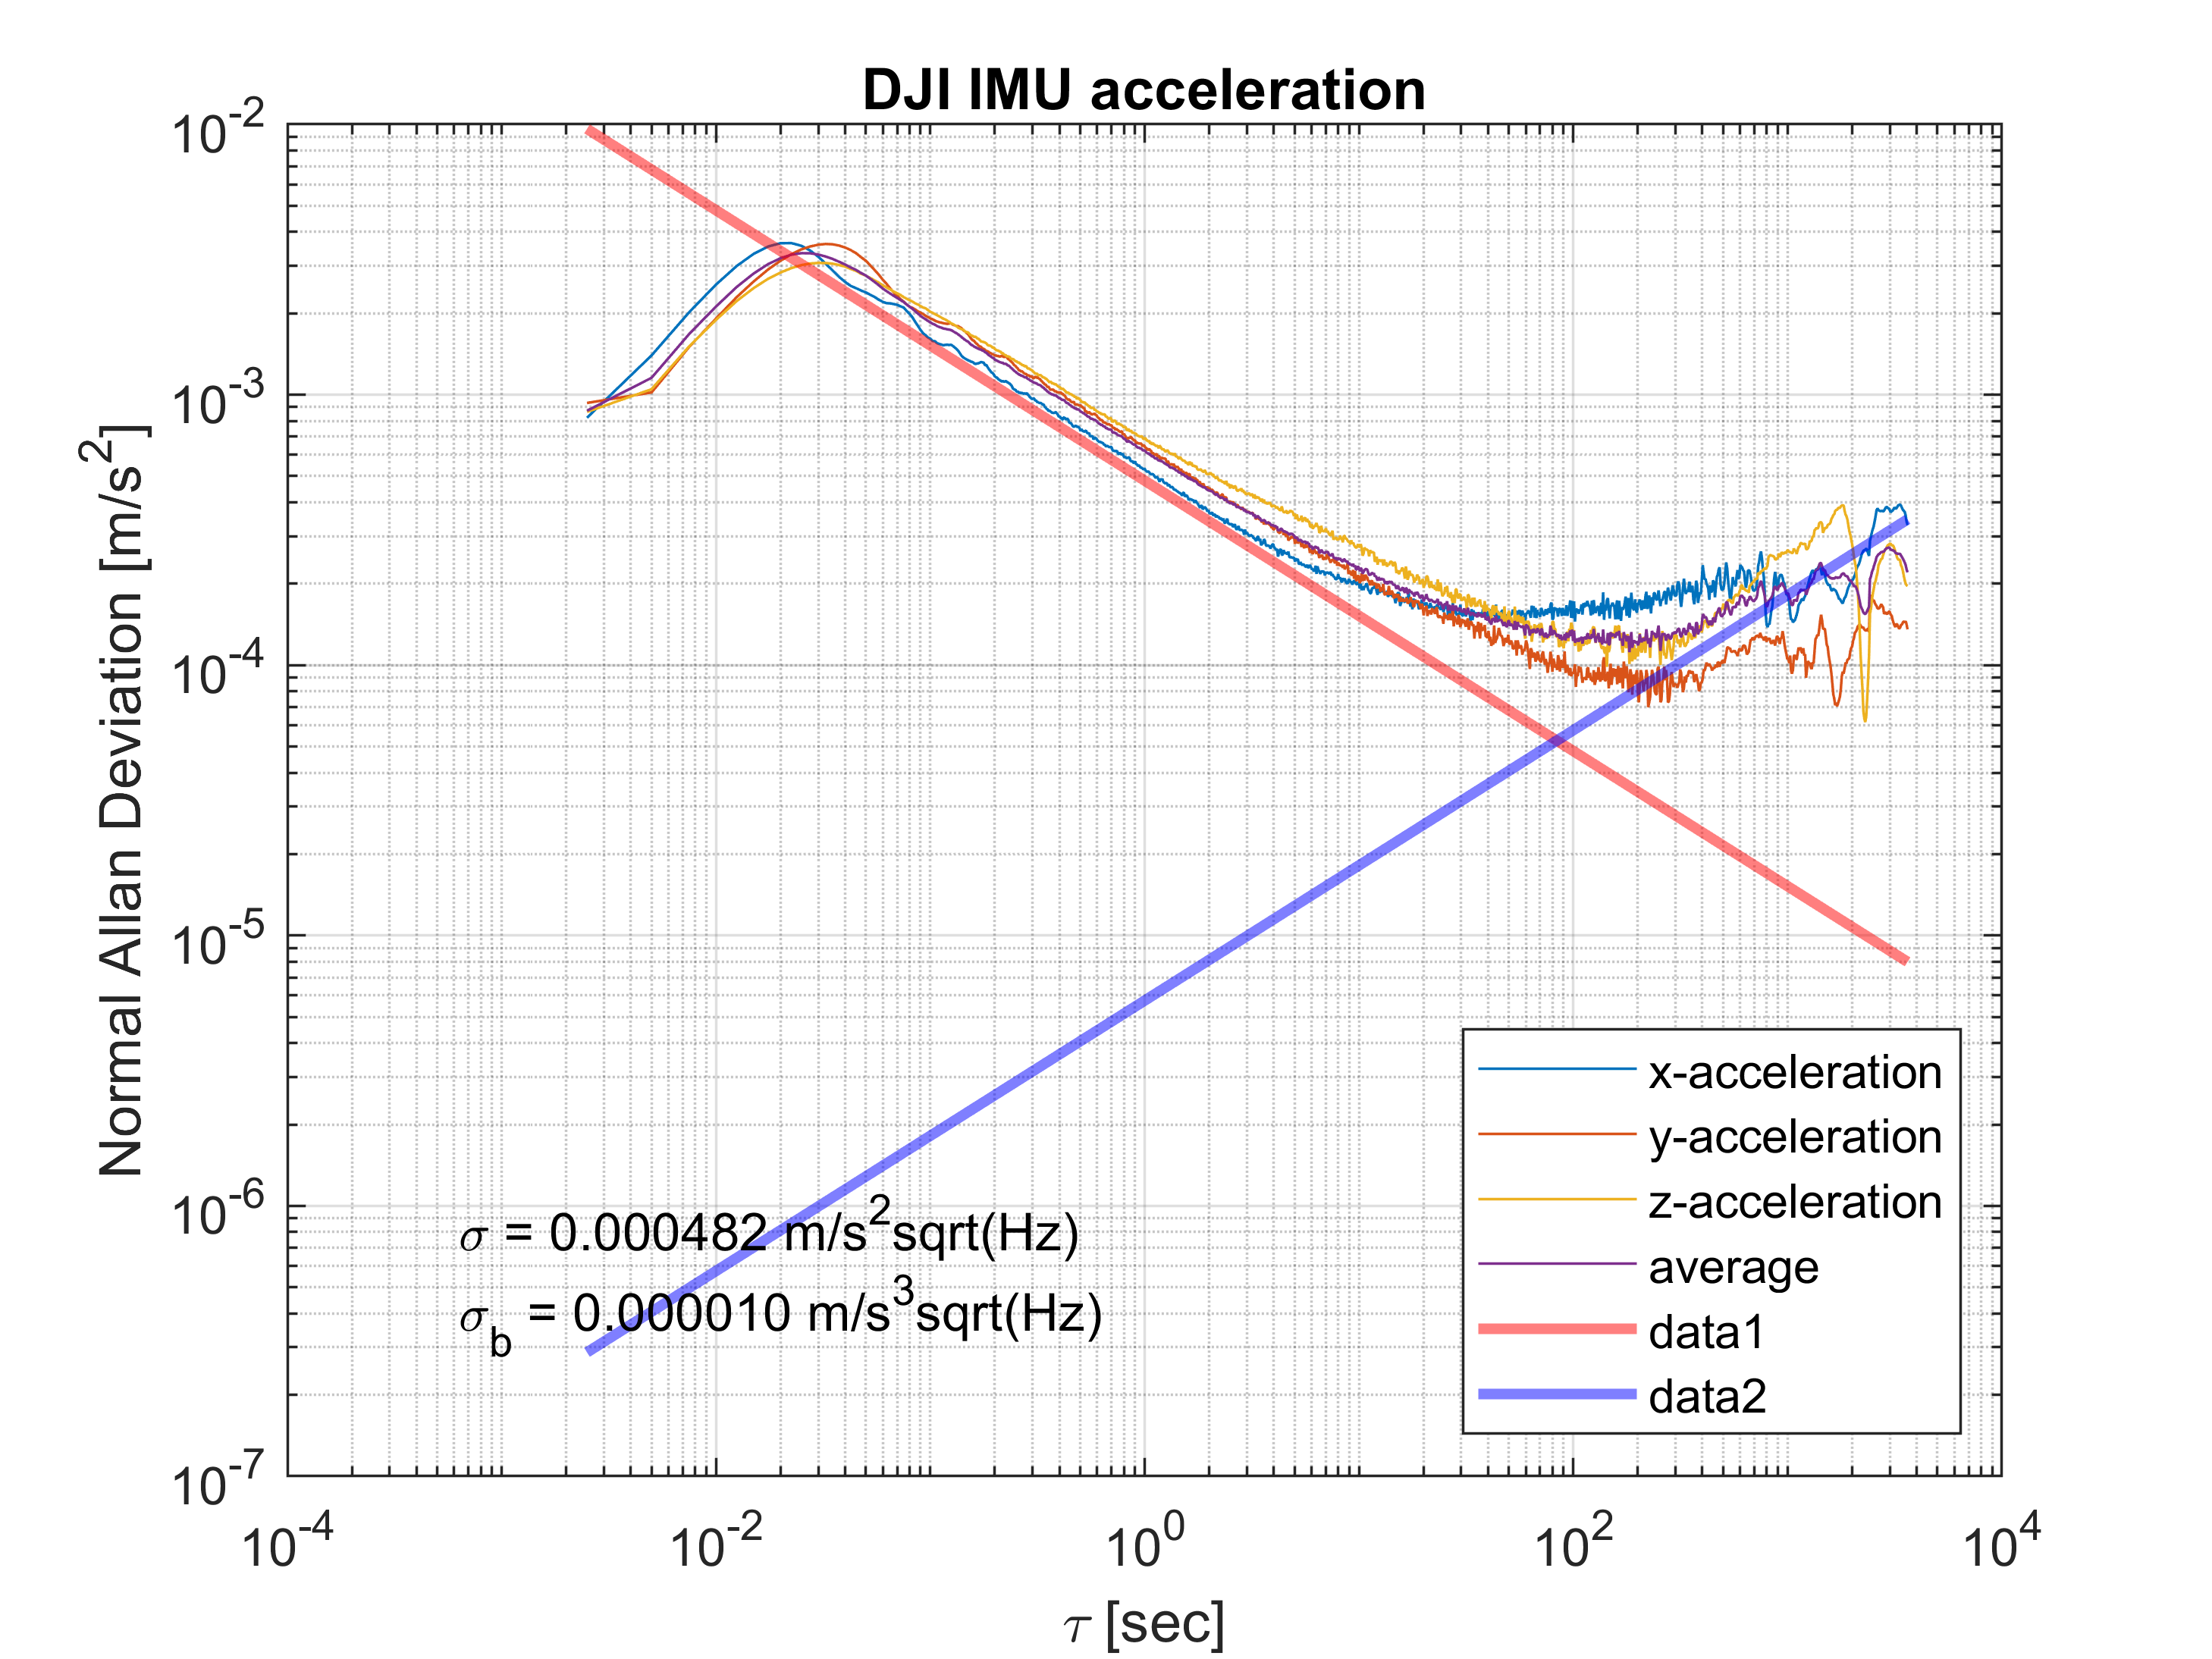
\includegraphics[scale=0.7]{Images/DJI_IMU_accel.png}
    \caption{Allan Deviation plot for Accelerometer}
    \label{fig:accel}
\end{figure}

\begin{figure}[h]
    \centering
    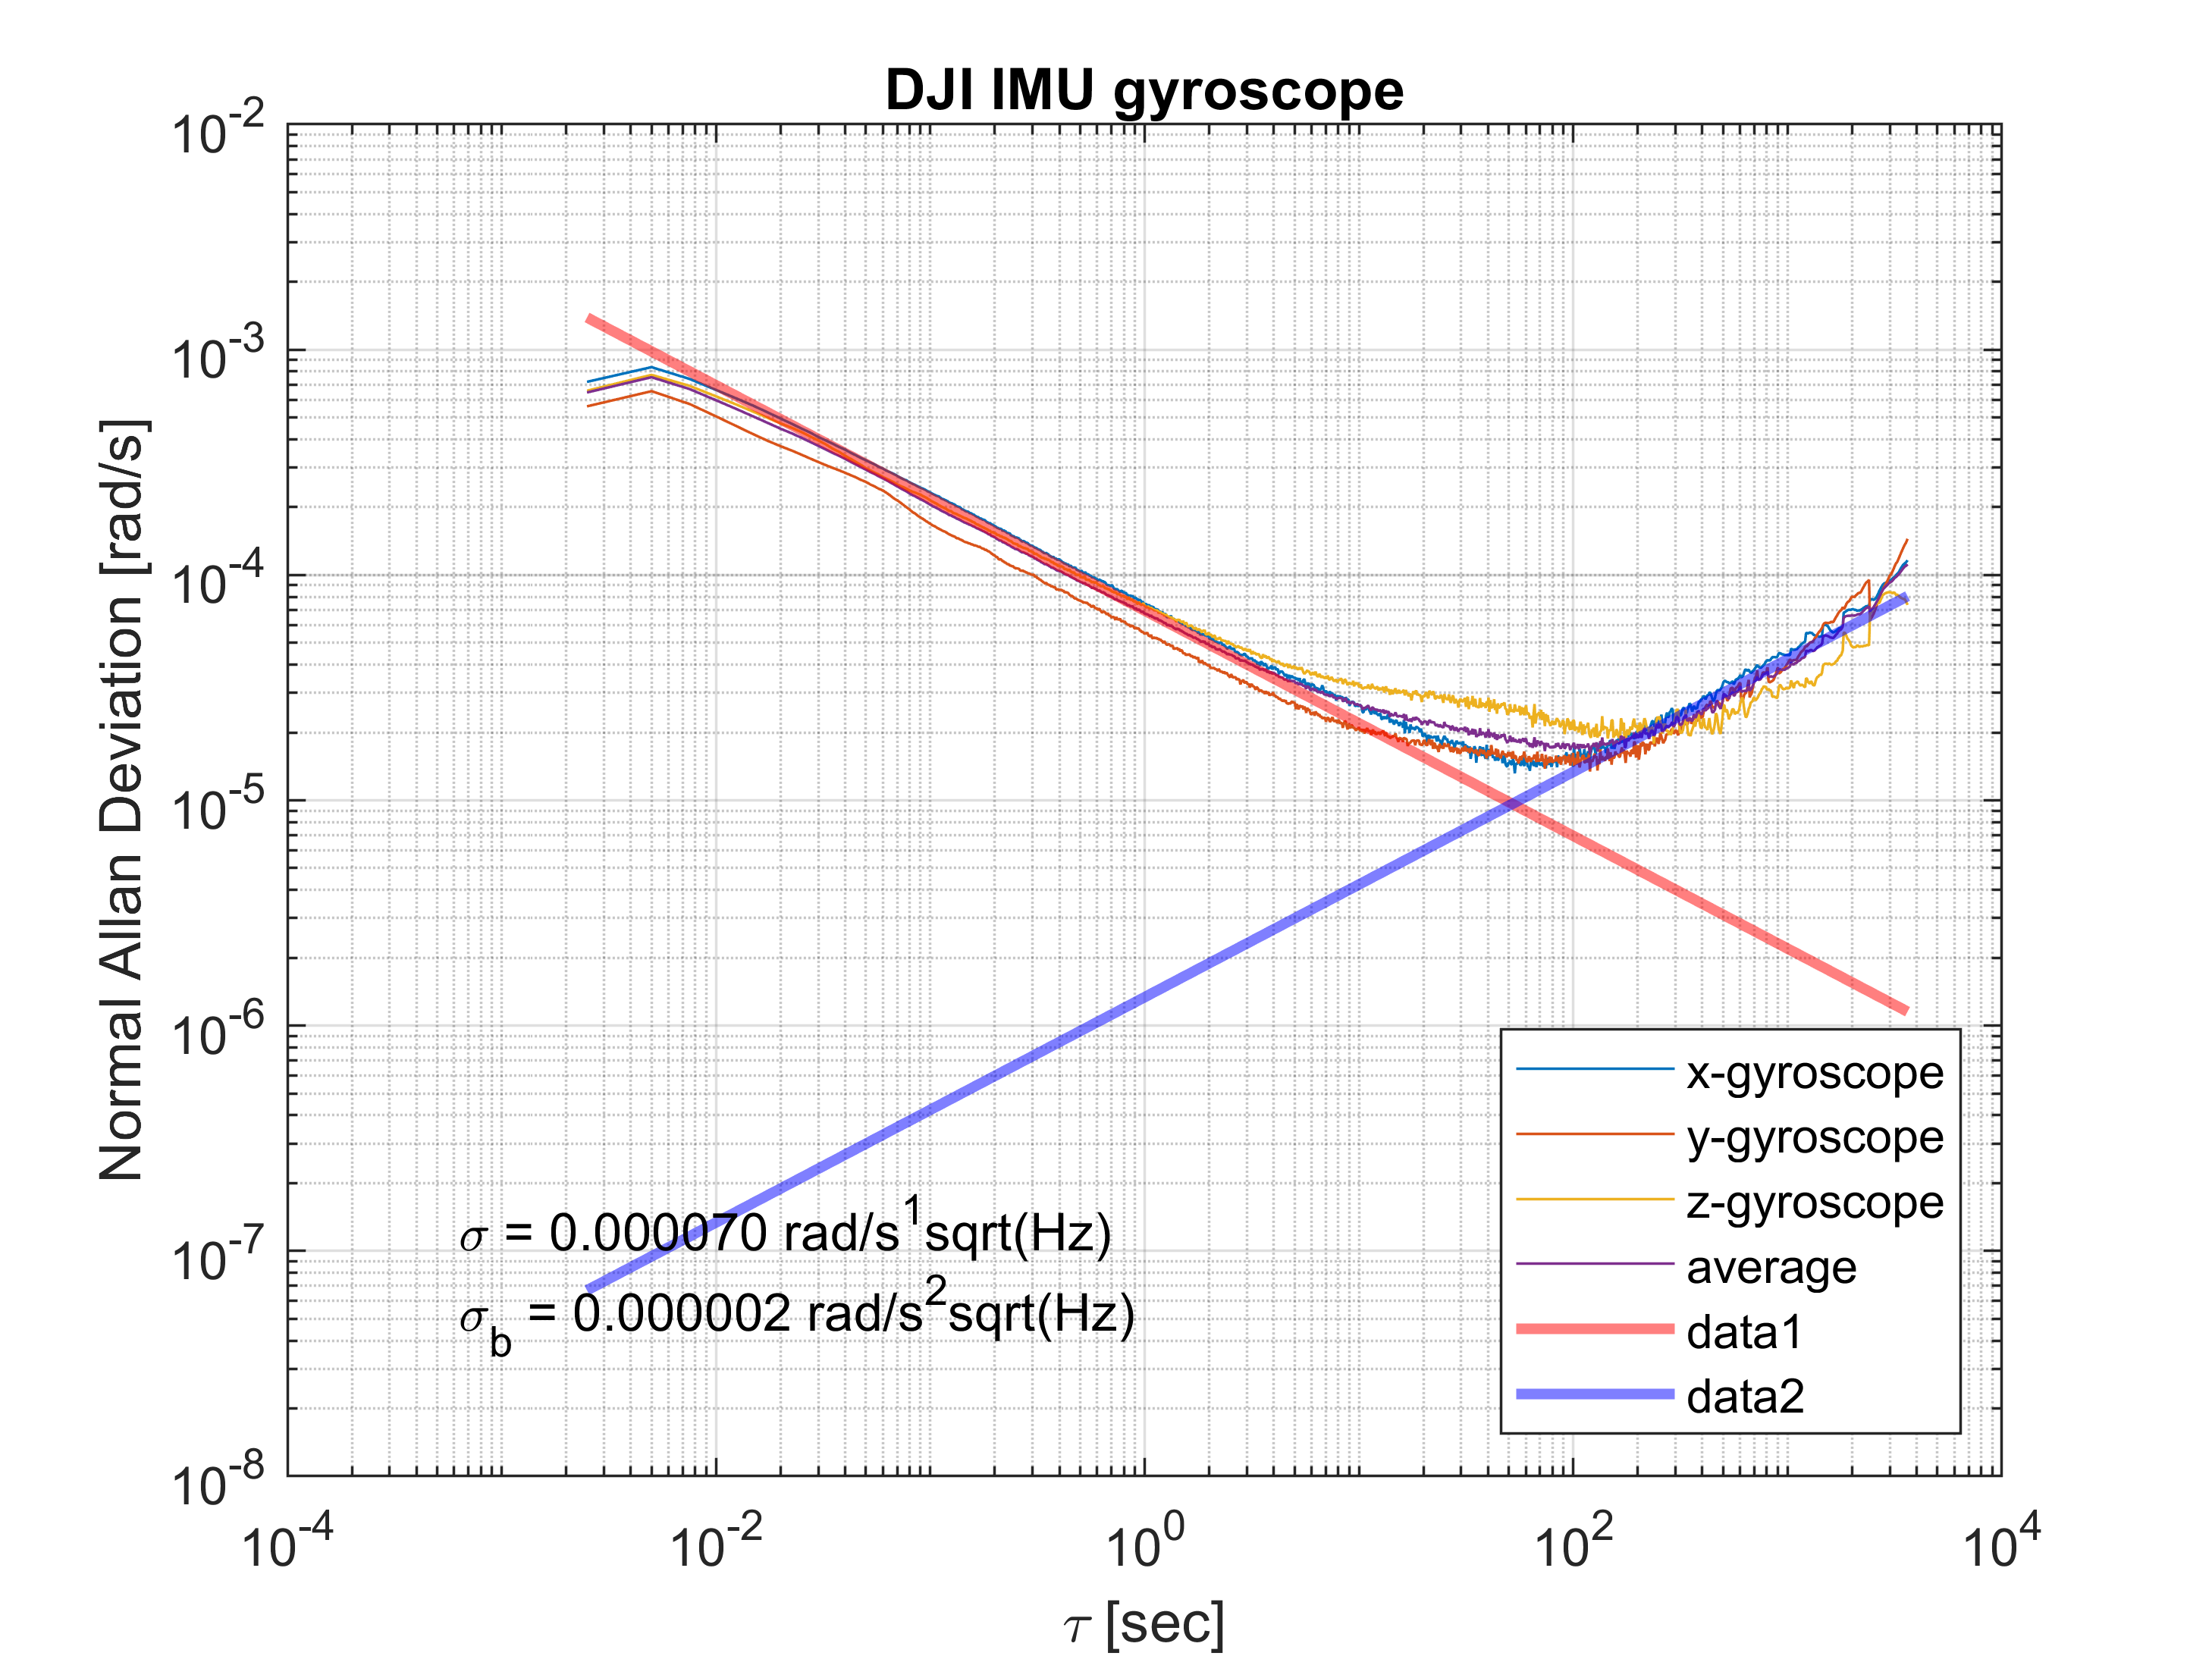
\includegraphics[scale=0.7]{Images/DJI_IMU_gyro.png}
    \caption{Allan Deviation plot for Gyroscope}
    \label{fig:gyro}
\end{figure}

Initially before recording, the drone was rotated, lifted and panned to excite the IMU sensor in all the axes. This helps in stabilizing any excitation error.The drone was also kept on a stationary platform and was undisturbed. Kalibr\_allan tool \cite{kalibrallan} was used for the calibration and the further steps for this process was followed as given in their official documentation.\\

The results obtained from this calibration were as follows:

\begin{itemize}
    \item Additive white noise for accelerometer, $\sigma\textsubscript{n}$ = 0.000482 $m/s\textsuperscript{2} . \sqrt{Hz}$
    \item Random walk or bias for accelerometer,  $\sigma\textsubscript{b}$ = 0.000010 $m/s\textsuperscript{3} . \sqrt{Hz}$
    \item Additive white noise for gyroscope, $\sigma\textsubscript{n}$ = 0.000070 $rad/s . \sqrt{Hz}$
    \item Random walk or bias for gyroscope,  $\sigma\textsubscript{b}$ = 0.000002 $rad/s\textsuperscript{2} . \sqrt{Hz}$
\end{itemize}

Also, the allan deviation plot was observed as shown in the Fig \ref{fig:accel} and Fig \ref{fig:gyro}. This process was performed multiple times to obtain the optimum values.

\subsection*{Calculating T\textsubscript{bc} matrix}
To synchronize the camera and body of the drone for the functioning of the VI-SLAM in general, a transformation matrix T\textsubscript{bc} is required by the system to calculate the camera poses. For this we used Kalibr camera-IMU calibration tool \cite{Kalibr}. The tool uses April Grid calibration schematic and a rosbag containing the movement of the drone in all the 6 axes of the IMU sensor with the camera feed. Further, the tool was used according the documentation and was able to generate T\textsubscript{bc} matrix and the value of the same is as follows:

\begin{align}
   T\textsubscript{bc} =
   \begin{bmatrix}
   -0.03292984 & -0.99925777 & -0.01998826 & 0.\\
  -0.06664725 & 0.02215003 & -0.99753071 & 0.\\
   0.99723306 & -0.03151636 & -0.06732718 & 0.\\
   0.     &     0.     &     0.     &     1.
   \end{bmatrix}
\end{align}

Since, the drone's main camera is installed with the gimbal, it was unable to fix the gimbal to single stationary position to record the movement of the drone. The gimbal auto-corrected the orientation of the camera with respect to the movement and rotation. We decided to use the FPV camera and a re-calibration was performed as explained in the Section \ref{sec:camcalib}.\\
\\
Intrinsic parameters and T\textsubscript{bc} values were updated in the settings file for the Visual Inertial SLAM. 

\section{vid\_orbslam3 node for Visual Inertial SLAM}
\label{sec:vidorbslam3VI-SLAM}
The vid\_orbslam3 node implementation from Visual SLAM was modified to work in Visual Inertial SLAM mode or in ORBSLAM3 terminologies, monocular-inertial mode. In this case, the node had to subscribe to IMU topic (/dji\_osdk\_ros/imu) from the drone. The node was accordingly developed to subscribe to both the topics at the same time and was made sure the camera frames and the IMU data were synchronized. The node was executed similar to Visual SLAM implementation mentioned in section \ref{sec:droneflight}. 

\subsection*{Observation}
Generally, the orbslam3 system takes a few frames to initialize itself and sets the first frame of the detection of key points as initial frame or the reference frame for the SLAM system. Every camera pose is determined with respect this initial frame. Interestingly, after every 2 frames the map was reset and the system was re-initialized for VI-SLAM. The main library code was debugged to find out what was the hindrance and reason for the map reset. It was found that there were not enough key points to consider the frame for the key frame list. Looking at this, it was evident that the keyframe graph is updated and a trajectory can be visualized only for a continuous tracking scenario.

\subsection*{Reasons for failure}
\label{subsec:reasonforfailure}
The above observations were finely investigated to find the reason for the failure of VI-SLAM of ORBSLAM3 on our drone. After trying multiple attempts of re-calibration and re-calculation of intrinsic and extrinsic parameters, the map reset was evident in all the attempts. On later stages of this investigation, one of the reasons for failure was found: ORBSLAM3 does not support rolling shutter cameras. Rolling shutter effects play a vital role in false point correspondences and key point extraction. Also, rolling shutter frame has a read out delay of in milli-seconds with at least 1/FPS ms. \\

Unfortunately, the main camera and the FPV camera on our drone DJI Matrice 210 RTK are rolling shutter cameras. It is convincing that, modeling the rolling shutter cameras for Visual SLAM or VI-SLAM is quite a task and even though when achieved the results are not satisfactory as compared to global shutter cameras. It was a good insight for us to plan the next stages of the task.

\newpage

\section{Testing other SLAM systems}
\label{sec:otherslamsystems}
Another attempt to implement VI-SLAM on the drone was made by employing other software implementations in the field of VI-SLAM. VINS-Mono \cite{qin2017vins} and open\_vins \cite{Geneva2020ICRA} were chosen to be tested on our platform with previously deduced IMU parameters and camera setup. Apparently, VINS-Mono supports rolling shutter cameras. But the performance analysis index using rolling shutter camera with VINS-Mono was rated the lowest among the other combinations of Global shutter camera and low to high end IMU sensors in their documentation.\\

VINS-Mono was installed on the local PC following the official documentation. A rosbag was recorded for the purpose of testing the VINS-Mono. The settings file for the VINS-Mono was similar to that of ORBSLAM3 and the corresponding fields in the settings file were updated with our findings from calibration. The example code was available for ROS environments and the VINS-Mono was tested with the recorded rosbag. Repeatedly, the Visual Inertial SLAM was failing here as well. VINS-Mono also considered the camera-IMU delay (t\textsubscript{r}) as an input in the settings file. Our calibration had an expected low delay time. For unknown reasons, the system was failing to track the key points after a couple of frames similar to ORBSLAM3.\\

Moving on, open\_vins was considered and installed on the same local PC following the official documentation. The open\_vins implementation does not explicitly support rolling shutter cameras but in the developer community there were a few attempts made to use rolling shutter camera for VI-SLAM. We attempted to perform VI-SLAM using open\_vins with our setup. Besides a lot trials in finding the right threshold to excite IMU at the drone's lift off to trigger the SLAM action to start (required by the open\_vins node), the position trajectory was drifting far away after a few seconds with drone being stationary held. From this observation, we were skeptical about the IMU intrinsic parameters because our values were really low. This results in highly sensitive sensor response while calculating displacement of the vehicle. A small movement of the drone would ramp up a higher response creating a huge drift in position trajectory and visualization. Also, in the settings file of the open\_vins for VI-SLAM, it was possible to specify the pixel noise to compensate the generic rolling shutter effect. We increased the pixel noise 5 to 10 times that of the standard value. Using this when tested, for some time the trajectory was close enough to expected results but down the line when there was a rapid movement of the vehicle, due to motion blur and highly sensitive IMU response would cause the drift. \\

Therefore, I would like to propose a conjecture from all the attempts made and observations analyzed: \textbf{Visual Inertial SLAM is not suitable for a setup whose camera is mounted on the gimbal with rolling shutter}. Visual Inertial SLAM needs a good IMU calibration with stable IMU response. Very low or very high response would lead to failure of accurate IMU calibration in turn leads to the failure of the Visual Inertial SLAM on autonomous aerial vehicles or drones which are bound to agility and undergo external influences affecting the movement of the vehicle. This conjecture is not perfect but sets a baseline for the future developments in this area. A rolling shutter model for VI-SLAM can be developed to handle all the failures as observed by our attempts. Visual Inertial SLAM is a good field to explore and has room for interesting results to come.

\subsubsection*{New attempt planned for the task}
To continue with Camera pose and keyframe trajectory estimation, we planned to drop the Visual Inertial SLAM on our setup. As the Visual SLAM was reasonable enough and tested to get the camera poses, it was decided to use the GPS data from the drone with Visual SLAM to achieve the task goals. Next sections in this report is designated as Part 2 of the task. The know-how and implementation of Visual SLAM with GPS data will be discussed in the further sections.

